\documentclass{article}
\usepackage[T1]{fontenc}
\usepackage{fontspec}
\usepackage{lmodern}
\usepackage{amsmath}
\usepackage[a4paper, left=3cm, right=3cm, bottom=2.5cm, top=2.5cm]{geometry}
\usepackage{graphicx}
\usepackage{listings}
\usepackage{svg}
\usepackage{lipsum}
\usepackage{caption}
\usepackage{array}
\usepackage{tabularx}


% clickable table of contents
\PassOptionsToPackage{hyphens}{url}\usepackage{hyperref}
\hypersetup{
colorlinks,
citecolor=black,
filecolor=black,
linkcolor=black
}

% Vertically center title
\usepackage{titling}
\renewcommand\maketitlehooka{\null\mbox{}\vfill}
\renewcommand\maketitlehookd{\vfill\null}

% Change table of contents title
\renewcommand*\contentsname{Inhaltsverzeichnis}

\usepackage{fancyhdr}
\usepackage{xcolor}
\pagestyle{fancy}

\fancyhead[L]{VanadiumCast}
\fancyfoot[L]{Silas Della Contrada \textcopyright\space2020}
\fancyfoot[C]{}
\fancyfoot[R]{\thepage}

\defaultfontfeatures{Ligatures=TeX}

%set line spacing
\usepackage{setspace}

% Custom font for SVGs
\newfontfamily\svgfont{Roboto}

\setsansfont{Roboto}
\newfontfamily\titlefont{Roboto}

\title{Dokumentation VanadiumCast}
\author{Silas Della Contrada}
\date{12/18/2020}

\setmainfont[Mapping=tex-text,AutoFakeSlant=0.2]{Roboto Slab}

\usepackage{titlesec}

\newfontfamily\headingfont[]{Roboto}
\titleformat*{\section}{\LARGE\bfseries\headingfont}
\titleformat*{\subsection}{\Large\bfseries\headingfont}
\titleformat*{\subsubsection}{\large\bfseries\headingfont}
\renewcommand{\maketitlehooka}{\headingfont}


\begin{document}

    \begin{titlingpage}
        \maketitle
    \end{titlingpage}

    \tableofcontents

    \newpage
    \linespread{1.25}


    \section{Vorwort}\label{sec:vorwort}

    Google Chromecast ist weit verbreitet, allerdings ist es nicht
    Open-Source und man ist gezwungen ein Google Chromecast oder ein Android
    TV als Ziel und entweder Chrome oder ein Android-Gerät als Quelle zu
    benutzen. Außerdem gibt es keine Möglichkeit den Desktop zu übertragen,
    wodurch eine potenziell gute Lösung eine große Nutzergruppe nicht
    anspricht. In diese Lücke fügt sich nun VanadiumCast ein.

    \subsection{Hinweis zur Formatierung}\label{sec:hinweis-zur-formatierung}

    Verweise zu Quellen und weiterführender Literatur sind mit einer
    dreistelligen Buchstabenkombination in eckigen Klammern dargestellt:

    \begin{quote}
        Bla bla bla\ldots{} {[}ExW{]}

        bla bla bla\ldots{} {[}ExB{]}
    \end{quote}
    Die Einträge im Literaturverzeichnis lauten dann wie folgt:

    \begin{quote}
    {[}
        ExW{]} \textit{Example website}: https://example.com/examplesite.html
        {[}2020-12-18{]}

        {[}ExB{]} Max Mustermann (2020), \textit{Example book}, Beispielverlag,
        ISBN: 1234567890
    \end{quote}

    \newpage


    \section{Projektidee}\label{sec:projektidee}

    Mit VanadiumCast kann man Videos und (in Zukunft) seinen Desktop an ein
    beliebiges Gerät übertragen, auf dem das Programm installiert ist. Es
    ist ähnlich einfach zu bedienen wie Chromecast, sodass es auch für
    technisch unbedarfte Personen gut nutzbar ist. Lediglich die Installation
    der Endgeräte ist deutlich schwieriger, da diese aber nur einmalig
    erfolgen muss, gibt es dort keine Probleme.

    Zudem ist geplant, dass VanadiumCast auf allen Desktop- und Mobilgeräten
    installiert und benutzt werden kann, sodass auch Handy -> Handy oder
    Desktop -> Handy Übertragungen möglich sind. Als Zielgerät eignet sich
    aktuell nur Laptops / PCs / Mini-PCs / Einplatinencomputer mit Intel-CPUs ab
    der 3. Generation mit iGPUs oder Nvidia-GPUs ab der GTX 8xx, als Quellgerät die
    gleichen Gerätetypen, jedoch werden hier Intel-CPUs ab der 4. Generation
    vorausgesetzt, da auf der Quelle mehr Leistung benötigt wird als auf dem
    Ziel. Es ist aber geplant beide Seiten zu optimieren und zu erweitern,
    sodass auch kleine SBCs wie ein Raspberry Pi oder Pine A64 als Ziel
    und/oder Quelle geeignet sind.

    Damit ist es dann auch möglich, ganze Schulen mit günstigen SBCs
    auszustatten, um Schülerinnen und Schülern sowie Lehrkräften
    Bildschirmübertragungen zu ermöglichen, ohne den komplizierten Weg über
    Miracast zu gehen, der nur an Fernsehern und in Kombination mit Android
    oder Windows 10 möglich ist. Da die Software nur im LAN kommuniziert,
    ist auch der Datenschutz gewährleistet, bei Google Chromecast werden
    hingegen Daten in die Google Cloud gesendet. Zudem lässt sich bei
    VanadiumCast die Übertragungsqualität einstellen, sodass man nicht
    darauf angewiesen ist, dass die Software die richtige auswählt.


    \section{Motivation}\label{sec:motivation}

    Weil ich persönlich keinen Google Chromecast kaufen wollte und man damit
    auch keine Videos von Linux aus streamen könnte, habe ich mir am Ende
    der Sommerferien 2020 überlegt, ob man nicht auch selbst eine Lösung
    dafür entwickeln könnte. Also habe ich mich im Internet über mögliche
    C++-Bibliotheken informiert und es wurde schnell klar, dass die sehr
    einfache Idee recht schwierig umzusetzen ist. Da ich zu diesem Zeitpunkt
    aber an keinem anderen Projekt gearbeitet hatte, nahm ich die
    Herausforderung an. Das gesamte Projekt ist ein
    ``learning-by-doing''-Projekt, das heißt, dass ich mich dann über Dinge
    informiere, wenn ich sie konkret benötige. Zum Beispiel habe ich mich
    zuerst mit FFmpeg bzw. den Libav-Bibliotheken auseinandergesetzt, um zu
    verstehen, wie man ein Video in C++ transkodieren kann.

    \newpage


    \section{Eine kurze Einführung in AV-Verarbeitung}\label{sec:eine-kurze-einführung-in-av-verarbeitung}

    \subsection{Videocodecs}\label{subsec:videocodecs}

    Videos werden nicht im Rohformat abgespeichert, da sie unkomprimiert
    sehr viel Platz verbrauchen. Für einen Spielfilm auf Bluray, d.h. 120
    min. Full HD mit 1 Byte pro Farbe und 24 Bildern pro Sekunde, sind das
    bereits:
    \[1920\ *\ 1080\ *\ 3B\ *\ 24\ *\ 120\ *\ 60s\ =\ 1,074,954,240,000\ B\ \approx\ 1,1\ TB\]
    Diese Menge an Speicherplatz möchte niemand für einen Film auf seiner
    Festplatte bereitstellen. Daher wurde 1988 der Kompressionsstandard
    H.261 festgelegt, dessen Nachfolger zum Veröffentlichungszeitpunkt immer
    den aktuellen Stand der Technik darstellten, aktuell sind das H.264/AVC
    und H.265/HEVC, welche auch in VanadiumCast zum Einsatz kommen. In GPUs
    stecken seit ca. 10 Jahren Videoprozessoren, die die CPU beim
    En-/Dekodieren von Videos entlasten, sodass weniger Energie verbraucht
    wird. Erst dadurch wird es möglich, auf Handys, Tablets etc. Video
    abzuspielen, da die Akkulaufzeit sonst zu gering wäre.

    \subsection{Audiocodecs}\label{subsec:audiocodecs}

    Bei Audiodaten ist das Problem recht ähnlich, und auch wenn man auf
    aktuellen SD-Karten mehrere Stunden unkomprimiertes Audio speichern
    kann, ist es meistens ausreichend und teilweise besser, Audio zu
    komprimieren, z.B. bei Streaming-Diensten wie Spotify, da mobile Daten
    meist teuer und limitiert sind. Ursprünglich gab es das Problem, dass
    man auf Walkmans nicht ausreichend Platz hatte, um mehrere Stunden Musik
    zu speichern, weswegen eine Arbeitsgruppe des Frauenhofer IIS in
    Zusammenarbeit mit einer anderen Universität, AT\&T Bell Labs und
    Thomson die MP3-Kodierung entwickelte. Dabei wird Platz gespart, indem
    durch die Anwendung von Psychoakustik gezielt Teile der Daten
    weggelassen oder verkleinert werden, die der Mensch normalerweise nicht
    wahrnimmt. Dadurch wird bei einer Bitrate von 192 kBit/s eine
    Kompressionsrate von 85\% gegenüber einer Audio-CD erzielt. Aktuellere
    Codecs wie AAC und Opus unterscheiden sich von MP3 im
    Kompressionsalgorithmus und der Qualität bei bestimmten Bitraten, sodass
    sie unterschiedlich gut für das Streaming geeignet sind. In VanadiumCast
    wird aktuell AAC verwendet, da es die gleiche Qualität wie MP3 bei
    geringerer Bitrate gewährleistet.

    \subsection{Containerformate}\label{subsec:containerformate}

    Ein Video- oder Audiocodec alleine reicht nicht aus, um eine Video mit
    Ton und eventuellen Untertiteln etc. abzuspeichern, daher gibt es
    Containerformate, durch die mehrere Video-/Audiospuren teilweise mit
    Untertiteln in einer Datei vereint werden. Die Auswahl des
    Containerformat hat nahezu keinen Einfluss auf die Dateigröße, sondern
    nur in den Möglichkeiten, welche Art von Daten enthalten sein können.
    Bekannte Beispiele sind das von Apple entwickelte und weit verbreitete
    MP4 oder das offene Matroska-Format, ersteres unterstützt nur Video- und
    Audiospuren, letzteres alle möglichen Spuren inklusive 3D-Inhalte und
    Menüs wie auf DVDs.

    \newpage


    \section{Umsetzung}\label{sec:umsetzung}

    \subsection{Bibliotheken und Frameworks}\label{subsec:bibliotheken-und-frameworks}

    Ursprünglich habe ich mich direkt mit FFmpeg und den Libav-Bibliotheken
    auseinandergesetzt, um den Transcoder umzusetzen, aber der Code des
    Transcoders wurde mit steigender Komplexität des Projekts nicht mehr
    verständlich, weswegen ich mich nach einer Alternative umgeschaut habe.
    Dabei bin ich auf das Qt-Plugin QtAV gestoßen, welche exakt die
    Funktionalität bietet, die ich benötige, und eine bessere API als ich
    sie jemals hätte schreiben können. Der Umstieg war recht einfach, da der
    Transcoder von QtAV lediglich ein Ein- und ein Ausgabegerät benötigt, in
    diesem Falle eine Datei und eine Netzwerkverbindung, und konfiguriert
    werden muss. Bei der Konfiguration bin ich auf einige Probleme gestoßen,
    da das Programm abstürzt oder sich aufhängt, wenn man die Konfiguration
    nicht auf die richtige Art und in der exakt richtigen Reihenfolge macht.
    Da QtAV aber einige Beispiele auf GitHub zur Verfügung stellt, konnte
    ich das Problem in relativ kurzer Zeit lösen. Aktuell bestehen noch
    Probleme mit der Audio-Übertragung, aber ich denke, dass auch die mit
    etwas Zeit lösbar sind.

    \subsubsection{Qt}\label{subsubsec:qt}

    Qt ist ein Anwendungsframework für C++ und Python, welches nahezu alle
    Funktionen für die Anwendungsentwicklung bereitstellt, z.B.
    Datenbank-Anbindung, Netzwerkkommunikation und GUIs. Darüber hinaus gibt
    es noch diverse Plugins von The Qt Company, also der Firma, die Qt
    entwickelt und vertreibt, z.B. für 3D-Darstellung, Diagramme etc.,
    sodass man in fast allen Fällen die benötigten Funktionen direkt in Qt
    findet. Sollte das wie bei mir nicht der Fall sein, existieren
    zahlreiche Plugins der Community, die häufig Open-Source und gut
    dokumentiert sind, die man sich dann herunterladen und installieren
    kann.

    In Qt gibt es zwei Möglichkeiten der prozessinternen Kommunikation, zum
    einen mit Signals und Slots und zum anderen mit Events. Diese beiden
    sollen im Folgenden kurz erläutert werden, sie in Gänze zu erklären,
    würde den Rahmen dieser Dokumentation bei weitem sprengen. Wer sich
    weiter mit Qt beschäftigen möchte, dem empfehle ich die Seite ``Qt for
    Beginners'' im Qt Wiki {[}QfB{]}.

    \paragraph{Signal-Slot-Prinzip}

    In Qt gibt es die Möglichkeit, in einer Klasse spezielle Methoden zu
    deklarieren, die Signale und Slots. Signale muss man nur deklarieren,
    d.h., sie erhalten keine Funktionalität vom Programmierer. Beim
    Kompilieren des Codes geht ein Programm namens Meta-Object-Compiler
    (MOC) durch alle Klassen, die Signale und/oder Slots enthalten oder
    benutzen und stattet diese entsprechend der spezifizierten Verbindungen
    mit Funktionalität aus, wodurch die Signale und Slots erst nutzbar
    werden. Diese Funktionalität ist ebenfalls sehr nützlich, wenn man
    mehrere parallel laufende Funktionen hat, die miteinander Daten
    austauschen müssen.

    Außerdem muss im Programm eine Event-Loop gestartet werden, d.h., es
    wird eine parallel laufende Funktion gestartet, die nichts anderes tut,
    als alle in die Event-Queue eingereihten Signale abzuarbeiten und die
    verbundenen Slots aufzurufen.

    \paragraph{Event-Prinzip}

    Auch Events werden von der Event-Loop bearbeitet, daher hat sie auch
    ihren Namen erhalten. Events werden \textbf{nur} bei Oberflächen
    benutzt, und arbeiten auf einer Ebene unter den Signalen und Slots. Sie
    werden ausgelöst, wenn der Benutzer im Fenster die Maus bewegt, mit ihr
    klickt, das Fenster vergrößert oder verkleinert, wenn das Fenster
    minimiert, maximiert oder in Vollbildmodus gesetzt wird. Es gibt viele
    weitere Eventtypen, siehe die API-Referenz zu Qt-Events {[}QER{]}.
    Da es nur vordefinierte Events gibt, kann man auch nur vordefininierte Event-Handler überschreiben.

    \paragraph{Oberflächen mit QML}
    Für Qt existieren zwei Möglichkeiten eine Oberfläche zu erstellen, eine davon ist die Qt Markup Language (QML).
    Mit QML kann man sehr schnell Oberflächen erstellen, da es vordefinierte Elemente, wie Knöpfe oder Text-Eingaben, gibt, die nur miteinander kombiniert werden müssen.
    Außerdem stehen drei Themes zur Auswahl: Material, das Standard Design unter Android 5 - 8, Universal, das Windows App Design, und Fusion, das Standard Qt Design.
    Direkte Funktionalität lässt sich per Javascript in QML einbetten, zudem ist es möglich, bestimmte, aus C++ zur Verfügung gestellte,
    Methoden aus QML aufzurufen, sodass Anwendungen mit QML meistens aus zwei Teilen bestehen, dem GUI und
    der eigentlichen Funktionalität der Anwendung, da C++ deutlich effizienter ist als Javascript.
    Zwischen QML und C++, wie auch zwischen einzelnen Elementen in QML, erfolgt die Kommunikation meist per Signal-Slot-Prinzip.
    Die Events werden bei QML-Oberflächen zwar auch generiert, aber von der QML-Engine ausgewertet, sodass in QML keine Events ankommen.

    \subsubsection{QtAV}\label{subsubsec:qtav}

    QtAV ist ein Plugin für Qt, das Funktionen wie A/V-Wiedergabe/-Transkodierung hinzufügt.
    Es gibt zwar ein Qt Multimedia Modul von The Qt Company, welches auf den GStreamer Bibliotheken basiert,
    aber nur die A/V-Wiedergabe und nicht Transkodieren oder Hardwarebeschleunigung unterstützt.
    Außerdem hat das QtAV-Plugin viel mehr Optionen als das Multimedia Modul,
    z.B. fehlt im Multimedia Modul die Möglichkeit, festzulegen,
    auf welche Art man das Video anzeigen möchte, ob in einem separaten Fenster oder so,
    dass es sich in die bestehende Oberfläche integriert.

    \newpage

    \subsection{Entwicklungsverlauf}\label{subsec:entwicklungsverlauf}
    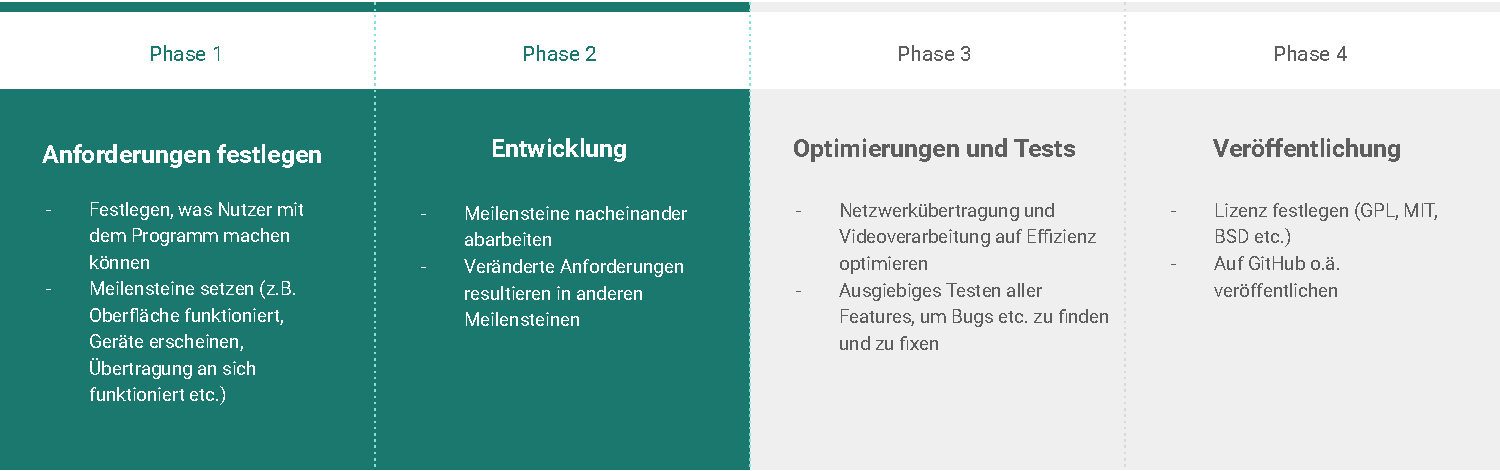
\includegraphics[width=\textwidth]{Progress.pdf}

    \subsubsection{Phase 1: Anforderungen festlegen}\label{subsubsec:phase-1:-anforderungen-festlegen}

    Zunächst müssen die Anforderungen an die Anwendung festgelegt werden, d.h. es wird festgelegt, was der Benutzer mit der Anwendung machen können soll.
    Dazu legt man sogenannte User Stories an, die beschreiben, was der Nutzer tun möchte.

    Die User Stories entsprechen hier den in der Abbildung erwähnten Meilensteinen.

    \paragraph{User Stories}
    \begin{enumerate}
        \item {Geräte im Netzwerk auflisten lassen}
        \item {Ein Gerät auswählen}
        \item {Datei als Quelle auswählen}
        \item {Ein Profil auswählen}
        \item {Stream starten}
        \item {Stream beenden}
        \item {Stream kontrollieren (Play/Pause, Vor-/Zurückspulen)}
        \item {Profile auf Kompatibilität testen lassen}
        \item {Desktop als Quelle auswählen}
    \end{enumerate}

    \subsubsection{Phase 2: Entwicklung}\label{subsubsec:phase-2:-entwicklung}

    Bei der Entwicklung arbeite ich die Meilensteine der Reihenfolge ab, da Meilensteine immer auf den vorhergehenden basieren.
    Wenn sich die Anforderungen ändern, z.B. die Möglichkeit den Desktop zu übertragen,
    werden diese abhängig von deren Voraussetzungen in die Liste Meilensteine eingereiht.
    Sollte die Anforderung neu sein, dann wird sie an die Liste der Meilensteine angehängt,
    sollte sich jedoch nur ein bestehender Meilenstein geändert haben, wird dieser zunächst bearbeitet,
    da es sein kann, dass dadurch die Implementationen der nachfolgenden Meilensteine geändert werden müssen.

    \subsubsection{Phase 3: Optimierungen und Tests}\label{subsubsec:phase-3:-optimierungen-und-tests}
    In dieser Phase ist geplant, die aktuell leistungsaufwändige Transkodierung effizienter zu machen
    und andere ineffiziente Anwendungsteile durch Tests ausfindig zu machen und zu beheben.
    Außerdem werden sowohl die gesamte Anwendung als auch die einzelnen Komponenten separat getestet,
    um Bugs zu finden und zu beheben.
    Das heißt zum einen, dass ich die gesamte Anwendung, in allen Varianten und Fehlermöglichkeiten testen werden,
    z.B. dass man während des Streams ein Seite per Taskmanager abbricht.
    Außerdem werden die einzelnen Komponenten durch Unit-Tests geprüft.

    Ein Unit-Test ist eine Sammlung von Methoden, die alle eine Komponente der Anwendung, aber verschiedene Szenarien, prüfen.
    Man muss so lange Fehler suchen und beheben, bis alle Tests erfolgreich durchlaufen werden.

    \subsubsection {Phase 4: Veröffentlichung}\label{subsubsec:phase-4:-veröffentlichung}
    Zunächst muss ich mich über die verschiedenen Open-Source Lizenzen informieren und eine auswählen.
    Danach werde ich das Projekt vermutlich auf GitHub veröffentlichen, sodass jeder Zugriff darauf hat und es benutzen kann.
    Da GitHub auch Features wie Issues bietet, können anderen Fehler oder auch Verbesserungsvorschläge dort einreichen,
    damit ich diese bearbeiten und gegebenenfalls Rückfragen stellen kann.
    Außerdem können dann Schulen VanadiumCast nutzen, sobald die Desktop-Übertragung implementiert ist,
    um den Schülerinnen, Schülern und Lehrkräften eine komfortable Möglichkeit zu bieten,
    im Unterricht den eigenen Bildschirm zu teilen.

    \newpage


    \section{Architektur}\label{sec:architektur}

    \subsection{Komponenten}\label{subsec:komponenten}

    \begin{figure}[!h]
        \centering
        {
        \svgfont
        \resizebox{\textwidth}{!}{\input{Components.pdf_tex}}
        }
        \caption*{Abb.\ref{subsec:komponenten}.1: Komponentendiagramm}
    \end{figure}

    Die Anwendung ist so strukturiert, dass sie leicht erweiterbar ist, z.B.
    kann man die Device-Komponente austauschen, wenn die Geräte per Bluetooth gesucht werden sollen.
    In der Streaming-Komponente muss in diesem Fall jedoch nichts geändert werden, wenn die
    Daten weiterhin über das Netzwerk übertragen werden sollen, solange die Geräte ihre IP-Adresse beim Scannen mit zurückgeben.
    Auch kann man die Sink-Komponente austauschen, wenn man z.B. die Ausgabe in eine Oberfläche integrieren möchte oder
    der Stream in eine Datei geschrieben statt angezeigt werden soll.

    \subsubsection{GUI (QML)}\label{subsubsec:gui-(qml)}

    \paragraph{Aufbau}
    Die Oberfläche der Anwendung ist in QML geschrieben, daher ist sie vom Backend
    (Backend $\hat=$ alles bis auf die Oberfläche und deren direkte Funktionalität wie "Knopfdruck -> Dateiauswahldialog")
    getrennt und kann auch nur über ein API-Objekt auf die Funktionen des Backends zugreifen.
    Sie ist nach dem KISS-Prinzip gestaltet (Keep It Simple, Stupid).
    Der Quellcode der Oberfläche ist in \texttt{src/res/gui} zu finden.

    \paragraph{Geräteauswahl}
    Hier ist die erste der drei Views zu sehen, die Geräteauswahl.
    Diese ist, wie jede andere View, so einfach wie möglich gehalten,
    es gibt nur die Liste der gefundenen Geräte und die nächsten Schritte am unteren Rand.
    Der nächste Schritt ist jedoch nur auswählbar, wenn ein Gerät ausgewählt wurde,
    damit der Stream nicht gestartet werden kann, wenn kein Gerät ausgewählt wurde,
    da dies würde zu einem Absturz des Programmes führen.
    \begin{figure} [!ht]
        \centering
        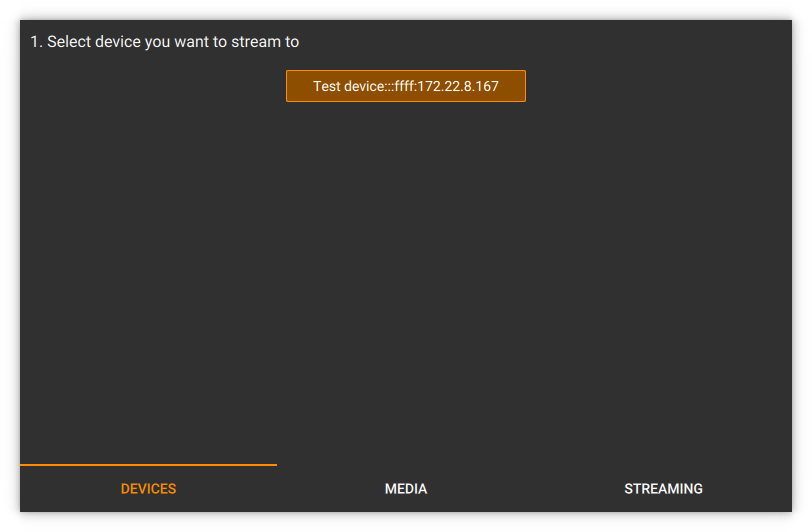
\includegraphics[height=6cm]{Devices.png}
        \caption*{Abb.\ref{subsubsec:gui-(qml)}.1: Geräteauswahl}
    \end{figure}

    \paragraph{Quellenauswahl}
    Zu sehen ist die Quellenauswahl in der aktuellen Fassung mit der Dateiauswahl.
    Es sind zum einen das Textfeld mit der direkten Eingabemöglichkeit einer URL (lokale Dateien starten mit \texttt{file://})
    Zudem gibt es einen Knopf zum Öffnen eines komfortableren Dateiauswahldialogs.
    Nachdem eine Datei ausgewählt wurde, wird sowohl die Videovorschau gestartet als auch der Knopf zum Starten des Streams freigeschaltet, um Fehler zu vermeiden.

    \begin{figure} [!ht]
        \centering
        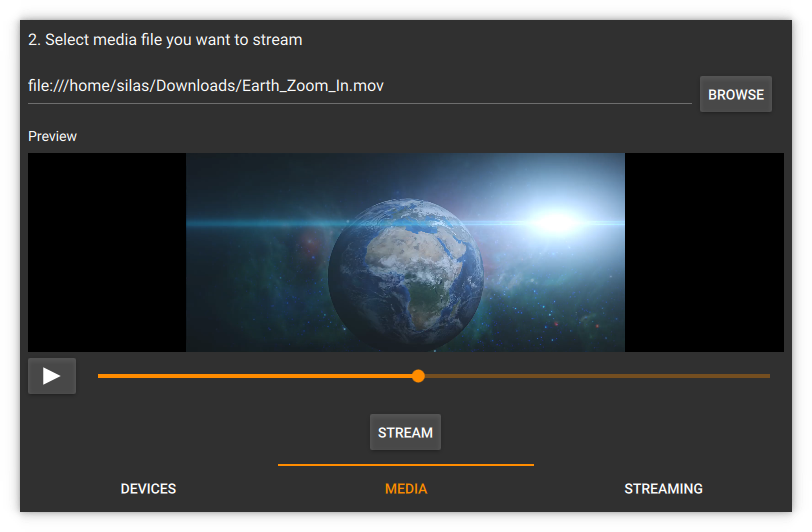
\includegraphics[height=6cm]{Media.png}
        \caption*{Abb.\ref{subsubsec:gui-(qml)}.2: Quellenauswahl}
    \end{figure}

    \newpage

    \paragraph{Wiedergabesteuerung}
    Die hier zu sehende Wiedergabesteuerung ist noch konzeptionell und ohne Funktion, d.h. es ist noch möglich, dass sich diese View im Rahmen der Entwicklung noch ändert.
    Aber auch hier ist das KISS-Prinzip deutlich erkennbar.
    Es gibt einen Knopf zum Pausieren/Fortsetzen der Wiedergabe,
    eine Anzeige der aktuellen Position und einen Schieberegler zum Setzen der Position.
    \begin{figure} [!ht]
        \centering
        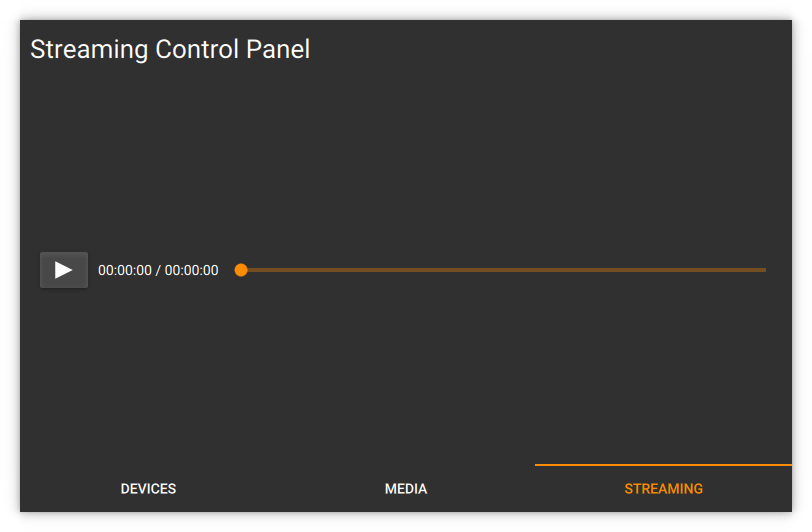
\includegraphics[height=6cm]{Streaming.png}
        \caption*{Abb.\ref{subsubsec:gui-(qml)}.3: Wiedergabesteuerung (konzeptionell)}
    \end{figure}

    \subsubsection{API (C++)}\label{subsubsec:api-(c++)}
    Die API die Schnittstelle zwischen QML und dem Backend.
    Dadurch kann man im Backend sehr einfach Komponenten austauschen, ohne in der Oberfläche etwas ändern zu müssen.
    In der API ist nur gerade so viel Anwendungslogik vorhanden, dass die einzelnen Komponenten verknüpft werden,
    der größte Teil ist in den einzelnen Komponenten.
    In der API ist z.B. die Funktion \texttt{startSource()} definiert,
    die lediglich der zuständigen Komponente Dateipfad und IP-Adresse des Ziels übergibt und die Komponente startet.

    \subsubsection{Devices (C++)}\label{subsubsec:devices-(c++)}

    \paragraph{DeviceScanner}
    Die Klasse \texttt{NetworkDeviceScanner} ist für das Scannen nach Geräten im Netzwerk zuständig.
    Die Funktion \texttt{run()} wird parallel zum Rest des Programms ausgeführt und verwaltet die gefundenen Geräte in einer Instanz der Klasse \texttt{NetworkDeviceDirectory}.
    Der Ablauf eines Scan-Vorgangs läuft wie folgt ab:
    \begin{enumerate}
        \item Senden eines UDP-Pakets an den Netzwerk-Broadcast
        \item Warten auf eingehende Pakete
        \item In jedem eingehenden Paket stehen der Name des antwortenden Geräts und die Senderadresse des Pakets ist die IP des Geräts
        \item Jedes so gefundene Gerät wird mit der Funktion \texttt{addDevice()} der Klasse \texttt{NetworkDeviceDirectory} zum Geräteverzeichnis hinzugefügt (siehe \textbf{DeviceDirectory})
        \item Am Ende jedes Scan-Vorgangs wird die Funktion \texttt{syncLists()} der Klasse \texttt{NetworkDeviceDirectory} verwendet, um die Geräteliste in der Oberfläche zu aktualisieren
    \end{enumerate}

    \paragraph{DeviceDirectory}
    Die Klasse \texttt{NetworkDeviceDirectory} verwaltet Instanzen der Klasse \texttt{NetworkDevice}, die in zwei Listen organisiert sind,
    in der einen stehen die Geräte des letzten vollständigen Scans, in der anderen die Geräte des aktuellen Scans.
    Diese Trennung ist dazu da, dass in \texttt{syncLists()} festgestellt werden kann, welche Geräte neu hinzugekommen sind und welche im aktuellen Scan fehlen.
    Außerdem wird in \texttt{syncLists()} für jedes Gerät, das nur in einer der beiden Listen vorhanden ist,
    entweder das Signal \texttt{addedDevice()} oder das Signal \texttt{removedDevice()} aufgerufen, welche mit einem Slot in QML verbunden sind,
    wo dann die Aktualisierung der Geräteliste in der Oberfläche stattfindet.
    Durch diese Methode werden nur so viele Aktualisierungen der Oberfläche durchgeführt, wie nötig sind.

    \paragraph{Device}
    Ein Gerät wird durch eine Instanz der Klasse \texttt{NetworkDevice} repräsentiert.
    Sie enthält den Namen und die IP-Adresse des Geräts.

    \subsubsection{Streaming (C++)}\label{subsubsec:streaming-(c++)}

    \paragraph{VideoTranscoder}
    Die Klasse \texttt{VideoTranscoder} enthält den für die Transkodierung zuständigen Code,
    der im wesentlichen aus dem Initialisieren und Starten des \texttt{AVTranscoder} aus dem QtAV-Plugin besteht.
    Beim Instanziieren der Klasse wird das Streaming-Profil übergeben, welches die Bitrate, FPS, Auflösung und den Videocodec angibt. (siehe Tabelle \ref{subsubsec:streaming-(c++)}.1)
    Aktuell ist das ausgewählt Profil als STANDARD im Code festgeschrieben, es ist aber geplant eine Auswahlmöglichkeit in die Oberfläche einzubauen.

    \begin{figure} [!ht]
        \begin{center}
            \texttt{
            \begin{tabularx}{\textwidth}{
            >{\raggedright\arraybackslash}X
            | >{\centering\arraybackslash}X
            | >{\centering\arraybackslash}X
            | >{\centering\arraybackslash}X
            | >{\centering\arraybackslash}X}
                Profilname & LOW      & STANDARD  & HIGH      & ULTRA     \\
                \hline
                Auflösung  & 1280x720 & 1920x1080 & 1920x1080 & 2560x1440 \\
                \hline
                FPS        & 30       & 30        & 60        & 60        \\
                \hline
                Bitrate    & 1 MBit/s & 5 MBit/s  & 10 MBit/s & 15 MBit/s \\
                \hline
                Videocodec & H.264    & H.264     & H.264     & H.265     \\
            \end{tabularx}
            }
        \end{center}
        \caption*{Tabelle \ref{subsubsec:streaming-(c++)}.1: Streaming-Profile}
        \label{fig:figure}
    \end{figure}

    \paragraph{StreamThread}
    Die Klasse \texttt{StreamThread} ist dafür zuständig, Transkoder und Netzwerkverbindung zu initialisieren und
    anschließend die Daten vom \texttt{VideoTranscoder} auf die Netzwerkverbindung zu schreiben.
    Dazu werden alle 2 ms alle Daten vom \texttt{VideoTranscoder} gelesen und auf die Netzwerkverbindung geschrieben.
    Außerdem steuert diese die Wiedergabe und sendet die entsprechenden Befehle auch an das Ziel,
    da z.B. erst die Wiedergabe auf dem Ziel pausiert werden muss, weil es sonst zu Fehlern kommt.
    Zudem wird die Klasse der Oberfläche die aktuelle Wiedergabeposition melden und diese auch von der Oberfläche steuern lassen.

    \subsubsection{Sink (C++)}\label{subsubsec:sink-(c++)}

    \paragraph{SinkHandler}
    Alles, bis auf die Darstellung an sich, ist in der Klasse \texttt{NetworkSinkHandler} implementiert,
    sowohl das Beantworten der Scan-Anfragen mit dem Namen, als auch das Steuern der Wiedergabe und das Senden/Empfangen von Befehlen.
    Beim Eingang einer Verbindungsanfrage wird zunächst die Oberfläche angewiesen, einen Dialog anzuzeigen, um den Benutzer zu fragen,
    ob die Verbindung angenommen oder abgelehnt werden soll.
    Währenddessen wartet der \texttt{NetworkSinkHandler} auf die Antwort, wenn diese negativ ausfällt, wird die Verbindung sauber geschlossen,
    wenn diese positiv ausfällt, dann werden Kontroll- und Datenverbindung aufgebaut, das \texttt{readyRead()}-Signal der Kontrollverbindung mit
    dem Slot \texttt{handleControl()} zum Bearbeiten von Kontrollbefehlen wie Pause, Weiter oder Stopp verbunden, der \texttt{VideoGuiLauncher} instanziiert und gestartet.
    Nach dem Absetzen des zeitverzögerten Startbefehls an den AVPlayer, tritt der \texttt{NetworkSinkHandler} in eine Schleife ein,
    die erst beim Beenden des Streams wieder verlassen wird, in welcher auf neue Daten auf der Netzwerkverbindung gewartet wird
    und diese Daten dann zum AVPlayer weitergeleitet werden.

    \paragraph{NetworkSinkTcpServer}
    Der \texttt{NetworkSinkTcpServer} ist eine von \texttt{QTcpServer} abgeleitete Klasse, die benötigt wird,
    da die Netzwerkverbindungen auf der Zielseite anders entgegengenommen werden müssen als \texttt{QTcpServer} ermöglicht.
    Dies liegt daran, dass nur der Thread\footnote{\label{footnoteThread}Ein Thread ist vereinfacht eine parallel zur aufrufenden Funktion laufende Funktion},
    in dem die Netzwerkverbindung erstellt wurde, diese auch nutzen kann.
    Da sich aber der \texttt{QTcpServer} für die Kontrollverbindungen nicht im selben Thread befindet wie der,
    in dem die \texttt{run()}-Methode des \texttt{NetworkSinkHandler} läuft,
    darf die Verbindung erst in der \texttt{run()}-Methode erstellt werden,
    auch wenn sie vorher entgegengenommen wurde.

    \paragraph{VideoGuiLauncher}
    Diese Klasse erstellt beim Empfang des Events vom Typ \texttt{QEvent::User}, welches für eigene Zwecke benutzt werden kann, das Ausgabefenster und den AVPlayer,
    welcher gleich darauf gestartet wird.
    Dieser Vorgang muss durch ein Event ausgelöst werden, da Oberflächenelemente nur im GUI-Thread\footnotemark[1] erstellt, verändert und gelöscht werden können und
    Events nur im GUI-Thread an Event-Handler\footnote[2]{Methode, die ein oder mehrere Events bearbeitet} ausgeliefert werden.

    \newpage


    \section{Anhang}

    \subsection{Flussdiagramm}\label{subsec:flussdiagramm}
    \textbf{Bitte heranzoomen, es ist ein SVG}
    \begin{figure}[!ht]
        \centering
        \def\svgwidth{\textwidth}
        \input{Flowchart.pdf_tex}
        \caption*{Abb.\ref{subsec:flussdiagramm}.1: Flussdiagramm}
        \label{fig:figureFlowChart}
    \end{figure}

    \newpage

    \subsection{Quellcode}
    Der Quellcode ist auf Anfrage hier verfügbar: \href{https://github.com/Katharineum/VanadiumCast}{GitHub}

    \newpage

    \subsection{Quellenverzeichnis}

    \subsubsection{\LaTeX betreffend}
    \url{https://www.overleaf.com/learn/latex/lists\#Ordered\_lists}\\
    \url{https://en.wikibooks.org/wiki/LaTeX/Source\_Code\_Listings}\\
    \url{https://tex.stackexchange.com/questions/73862/how-can-i-make-a-clickable-table-of-contents}\\
    \url{https://tex.stackexchange.com/questions/2099/how-to-include-svg-diagrams-in-latex}\\
    \url{https://tex.stackexchange.com/questions/373767/get-section-number-if-referencing-a-subsection-instead-of-subsection-number}\\
    \url{https://tex.stackexchange.com/questions/25249/how-do-i-use-a-particular-font-for-a-small-section-of-text-in-my-document}\\
    \url{https://tex.stackexchange.com/questions/196562/scaling-an-input-within-a-subfigure}\\
    \url{https://tex.stackexchange.com/questions/24840/use-courier-font-inline-on-text}\\
    \url{https://tex.stackexchange.com/questions/170080/how-do-you-write-the-estimate-equal-sign}\\
    \url{https://tex.stackexchange.com/questions/77809/how-do-i-remove-white-space-before-or-after-the-figures-and-tables/77811}\\
    \url{https://tex.stackexchange.com/questions/117151/undefined-control-sequence-and-chapter-error}\\
    \url{https://tex.stackexchange.com/questions/21795/how-to-remove-figure-label}\\
    \url{https://www.overleaf.com/learn/latex/tables}\\
    \url{https://tex.stackexchange.com/questions/341205/what-is-the-difference-between-tabular-tabular-and-tabularx-environments}\\
    \url{https://tex.stackexchange.com/questions/116534/lstlisting-line-wrapping/116572}\\
    \url{https://www.overleaf.com/learn/latex/footnotes}\\
    \url{https://tex.stackexchange.com/questions/35043/reference-different-places-to-the-same-footnote}\\
    \url{https://tex.stackexchange.com/questions/18507/change-font-of-document-title}\\
    \url{https://www.overleaf.com/learn/latex/sections\_and\_chapters}\\
    \url{https://tex.stackexchange.com/questions/10138/change-section-fonts}\\
    \url{https://www.fontsquirrel.com/fonts/roboto-slab}\\
    \url{https://tex.stackexchange.com/questions/3159/how-do-i-get-fake-slant-italics-with-xelatex}\\
    \url{https://tex.stackexchange.com/questions/2099/how-to-include-svg-diagrams-in-latex}\\
    \url{https://tex.stackexchange.com/questions/73862/how-can-i-make-a-clickable-table-of-contents}\\
    \url{https://en.wikibooks.org/wiki/LaTeX/Source\_Code\_Listings}\\
    \url{https://www.overleaf.com/learn/latex/lists\#Ordered\_lists}\\

    \subsubsection{Programmieren betreffend}
    \textbf{Die folgenden Quellen wurden alle im November 2020 aufgerufen}\\
    \url{https://forum.qt.io/topic/108139/qttest-test-multiple-classes}\\
    \url{https://www.qtcentre.org/threads/65673-when-QBuffer-emits-readyRead-signal}\\
    \url{https://forum.qt.io/topic/96771/how-to-test-class-with-signals-with-qtest-and-qsignalspy}\\
    \url{https://stackoverflow.com/questions/32290083/how-to-test-signal-slot-connections-with-qtest}\\
    \url{https://www.jetbrains.com/help/clion/qt-tutorial.html}\\
    \url{https://de.slideshare.net/m3xican/unit-testing-with-qt-test}\\
    \url{http://blog.davidecoppola.com/2017/11/cpp-unit-testing-with-qt-test-advanced/}\\
    \url{https://stackoverflow.com/questions/63948867/repetition-of-test-results-of-qt-test-in-qtcreator}\\
    \url{https://stackoverflow.com/questions/47998347/test-method-with-signals-and-slots}\\
    \url{https://stackoverflow.com/questions/21606125/qt-event-loop-and-unit-testing}\\
    \url{https://www.qtcentre.org/threads/65673-when-QBuffer-emits-readyRead-signal}\\
    \url{http://blog.davidecoppola.com/2017/11/cpp-unit-testing-with-qt-test-introduction/}\\
    \url{https://stackoverflow.com/questions/25431184/qt-slot-testing}\\
    \url{https://forum.qt.io/topic/96771/how-to-test-class-with-signals-with-qtest-and-qsignalspy}\\
    \url{https://stackoverflow.com/questions/32290083/how-to-test-signal-slot-connections-with-qtest}\\
    \url{https://forum.qt.io/topic/81919/using-mocks-with-networking}\\
    \url{https://stackoverflow.com/questions/40404331/subclassing-qiodevice-by-overriding-non-virtual-methods}\\
    \url{https://wiki.qt.io/Unit\_Testing}\\
    \url{https://stackoverflow.com/questions/4753845/build-qt-tests-with-cmake}\\
    \url{https://stackoverflow.com/questions/21606125/qt-event-loop-and-unit-testing/22951970}\\
    \url{https://www.ics.com/webinars/qt-test-driven-development-using-google-test-google-mock-video-demand}\\
    \url{https://stackoverflow.com/questions/39574360/google-testing-framework-and-qt}\\
    \url{https://forum.qt.io/topic/74176/using-google-test-with-qtcreator-and-autotest-plugin}\\
    \url{https://wiki.qt.io/Simple\_Crypt\_IO\_Device}\\
    \url{https://wiki.qt.io/Custom\_IO\_Device}\\
    \url{https://stackoverflow.com/questions/3549540/google-test-fixtures}\\
    \url{https://stackoverflow.com/questions/29297054/segmentation-fault-with-qhostaddress}\\
    \url{https://forum.qt.io/topic/91629/sos-undefined-reference-to-vtable-for-class-name}\\
    \url{https://forum.qt.io/topic/15171/warning-no-relevant-classes-found-no-output-generated}\\
    \url{https://lists.qt-project.org/pipermail/qt-interest-old/2010-April/021985.html}\\
    \url{https://stackoverflow.com/questions/57146235/opt-project-qt-spreadsheet-cell-h0-note-no-relevant-classes-found-no-output}\\
    \url{https://www.qtcentre.org/threads/19122-Warning-No-relevant-classes-found}\\
    \url{https://www.qtforum.de/viewtopic.php?t=9323}\\
    \url{https://forum.qt.io/topic/105770/moc-cpp-generation-fails-with-no-relevant-classes-found-no-output-generated}\\
    \url{https://lizardo.wordpress.com/2009/04/24/undefined-reference-to-vtable-for-errors-in-qt-derived-classes/}\\
    \url{https://stackoverflow.com/questions/14010922/qt-undefined-reference-to-vtable}\\
    \url{https://www.geeksforgeeks.org/friend-class-function-cpp/}\\
    \url{https://en.cppreference.com/w/cpp/language/friend}\\
    \url{https://stackoverflow.com/questions/4774291/q-object-throwing-undefined-reference-to-vtable-error}\\

    \subsection{Weiterführende Literatur}
    {[}QfB{]} Qt for Beginners: \url{https://wiki.qt.io/Qt\_for\_Beginners [12/2020]}\\
    {[}QER{]} QEvent Types: \url{https://doc.qt.io/qt-5/qevent.html\#Type-enum [12/2020]}\\


\end{document}
